\documentclass[11pt]{article}

\usepackage{amsmath,amssymb,amsfonts}
\usepackage{graphicx}
\usepackage{xcolor}
\usepackage{tikz}
\usepackage{pgfplots}
\usepackage{pgfplotstable}
\usepackage[many]{tcolorbox}
\usepackage{booktabs}
\usepackage{geometry}
\usepackage{multicol}

\geometry{margin=1in}

% Import our color scheme and plot styles
% ===================================
% COLOR SCHEME DEFINITIONS
% ===================================
% This file defines a consistent color palette for the entire book
% To use, include this file in book.tex with % ===================================
% COLOR SCHEME DEFINITIONS
% ===================================
% This file defines a consistent color palette for the entire book
% To use, include this file in book.tex with % ===================================
% COLOR SCHEME DEFINITIONS
% ===================================
% This file defines a consistent color palette for the entire book
% To use, include this file in book.tex with \input{book-sections/color-scheme.tex}

% Define primary colors
\definecolor{primary}{RGB}{31, 119, 180}       % Blue
\definecolor{secondary}{RGB}{255, 127, 14}     % Orange
\definecolor{tertiary}{RGB}{44, 160, 44}       % Green
\definecolor{quaternary}{RGB}{214, 39, 40}     % Red
\definecolor{quinary}{RGB}{148, 103, 189}      % Purple
\definecolor{senary}{RGB}{140, 86, 75}         % Brown
\definecolor{septenary}{RGB}{227, 119, 194}    % Pink
\definecolor{octonary}{RGB}{127, 127, 127}     % Gray
\definecolor{nonary}{RGB}{188, 189, 34}        % Olive
\definecolor{denary}{RGB}{23, 190, 207}        % Cyan

% Define light versions for fills and backgrounds
\definecolor{primaryLight}{RGB}{174, 199, 232}
\definecolor{secondaryLight}{RGB}{255, 187, 120}
\definecolor{tertiaryLight}{RGB}{152, 223, 138}
\definecolor{quaternaryLight}{RGB}{255, 152, 150}
\definecolor{quinaryLight}{RGB}{197, 176, 213}
\definecolor{senaryLight}{RGB}{196, 156, 148}
\definecolor{septenaryLight}{RGB}{247, 182, 210}
\definecolor{octonaryLight}{RGB}{199, 199, 199}
\definecolor{nonaryLight}{RGB}{219, 219, 141}
\definecolor{denaryLight}{RGB}{158, 218, 229}

% Define dark versions for text and lines
\definecolor{primaryDark}{RGB}{17, 63, 96}
\definecolor{secondaryDark}{RGB}{179, 89, 10}
\definecolor{tertiaryDark}{RGB}{22, 80, 22}
\definecolor{quaternaryDark}{RGB}{136, 22, 22}
\definecolor{quinaryDark}{RGB}{94, 66, 121}
\definecolor{senaryDark}{RGB}{85, 52, 45}
\definecolor{septenaryDark}{RGB}{143, 75, 122}
\definecolor{octonaryDark}{RGB}{64, 64, 64}
\definecolor{nonaryDark}{RGB}{104, 104, 18}
\definecolor{denaryDark}{RGB}{14, 115, 124}

% ===================================
% TCOLORBOX STYLES
% ===================================

% Reset tcolorbox definitions with the new colors
\newtcolorbox{definitionbox}[1][]{
    enhanced,
    colback=primaryLight!60!white,
    colframe=primary!75!black,
    fonttitle=\bfseries,
    coltitle=white,
    attach boxed title to top left={yshift=-2mm, xshift=5mm},
    boxed title style={colback=primary!75!black},
    title=Definition,
    #1
}

\newtcolorbox{equationbox}[1][]{
    enhanced,
    colback=secondaryLight!60!white,
    colframe=secondary!75!black,
    fonttitle=\bfseries,
    breakable,
    coltitle=white,
    attach boxed title to top left={yshift=-2mm, xshift=5mm},
    boxed title style={colback=secondary!75!black},
    title=Equation,
    #1
}

\newtcolorbox{examplebox}[1][]{
    enhanced,
    colback=tertiaryLight!60!white,
    colframe=tertiary!75!black,
    fonttitle=\bfseries,
    coltitle=white,
    attach boxed title to top left={yshift=-2mm, xshift=5mm},
    boxed title style={colback=tertiary!75!black},
    title=Example,
    #1
}

\newtcolorbox{notebox}[1][]{
    enhanced,
    colback=quinaryLight!60!white,
    colframe=quinary!75!black,
    fonttitle=\bfseries,
    coltitle=white,
    attach boxed title to top left={yshift=-2mm, xshift=5mm},
    boxed title style={colback=quinary!75!black},
    title=Note,
    #1
}

% ===================================
% TIKZ AND PGFPLOTS STYLES
% ===================================

% TikZ styles
\tikzset{
    concept/.style={
        draw=primary,
        fill=primaryLight,
        rounded corners,
        thick,
        align=center
    },
    process/.style={
        draw=secondary,
        fill=secondaryLight,
        rectangle,
        thick,
        align=center
    },
    decision/.style={
        draw=tertiary,
        fill=tertiaryLight,
        diamond,
        thick,
        align=center
    },
    data/.style={
        draw=quaternary,
        fill=quaternaryLight,
        cylinder,
        thick,
        align=center
    },
    note/.style={
        draw=quinary,
        fill=quinaryLight,
        cloud,
        cloud puffs=15,
        thick,
        align=center
    },
    arrow/.style={
        ->,
        >=stealth,
        thick
    }
}

% PGFPlots styles
\pgfplotscreateplotcyclelist{conceptcolors}{
    {primary, mark=*, thick, mark options={fill=primary}},
    {secondary, mark=square*, thick, mark options={fill=secondary}},
    {tertiary, mark=triangle*, thick, mark options={fill=tertiary}},
    {quaternary, mark=diamond*, thick, mark options={fill=quaternary}},
    {quinary, mark=pentagon*, thick, mark options={fill=quinary}},
    {senary, mark=*, thick, mark options={fill=senary}},
    {septenary, mark=square*, thick, mark options={fill=septenary}},
    {octonary, mark=triangle*, thick, mark options={fill=octonary}},
    {nonary, mark=diamond*, thick, mark options={fill=nonary}},
    {denary, mark=pentagon*, thick, mark options={fill=denary}}
}

% ===================================
% CONCEPT-SPECIFIC COLORS
% ===================================

% Assign consistent colors to specific concepts
% These can be used across diagrams to ensure the same concept has the same color

% Survival functions and models
\colorlet{survivalFunctionColor}{primary}
\colorlet{hazardFunctionColor}{secondary}
\colorlet{censoringColor}{quaternary}
\colorlet{kaplameierColor}{tertiary}

% Model types
\colorlet{dsmColor}{quinary}
\colorlet{mensaColor}{septenary}
\colorlet{deephitColor}{senary}

% Loss functions
\colorlet{likelihoodLossColor}{primary}
\colorlet{rankingLossColor}{secondary}
\colorlet{regressionLossColor}{tertiary}
\colorlet{classificationLossColor}{quaternary}
\colorlet{auxiliaryLossColor}{quinary}

% Events
\colorlet{event1Color}{primary}
\colorlet{event2Color}{secondary}
\colorlet{event3Color}{tertiary}
\colorlet{event4Color}{quaternary}

% Risk groups
\colorlet{lowRiskColor}{tertiary}
\colorlet{mediumRiskColor}{primary}
\colorlet{highRiskColor}{quaternary}

% ===================================
% USAGE EXAMPLES
% ===================================
%
% For tcolorbox:
% \begin{definitionbox}[title=Custom Title]
% Content
% \end{definitionbox}
%
% For TikZ:
% \begin{tikzpicture}
%   \node[concept] (a) {Concept};
%   \node[process] (b) at (2,0) {Process};
%   \draw[arrow] (a) -- (b);
% \end{tikzpicture}
%
% For PGFPlots:
% \begin{tikzpicture}
%   \begin{axis}[cycle list name=conceptcolors]
%     \addplot coordinates {(0,0) (1,1) (2,4)};
%     \addplot coordinates {(0,0) (1,2) (2,3)};
%   \end{axis}
% \end{tikzpicture}
%
% For concept-specific colors:
% \begin{tikzpicture}
%   \draw[survivalFunctionColor, thick] plot coordinates {(0,1) (1,0.8) (2,0.6)};
%   \draw[hazardFunctionColor, thick] plot coordinates {(0,0.2) (1,0.4) (2,0.6)};
% \end{tikzpicture}


% Define primary colors
\definecolor{primary}{RGB}{31, 119, 180}       % Blue
\definecolor{secondary}{RGB}{255, 127, 14}     % Orange
\definecolor{tertiary}{RGB}{44, 160, 44}       % Green
\definecolor{quaternary}{RGB}{214, 39, 40}     % Red
\definecolor{quinary}{RGB}{148, 103, 189}      % Purple
\definecolor{senary}{RGB}{140, 86, 75}         % Brown
\definecolor{septenary}{RGB}{227, 119, 194}    % Pink
\definecolor{octonary}{RGB}{127, 127, 127}     % Gray
\definecolor{nonary}{RGB}{188, 189, 34}        % Olive
\definecolor{denary}{RGB}{23, 190, 207}        % Cyan

% Define light versions for fills and backgrounds
\definecolor{primaryLight}{RGB}{174, 199, 232}
\definecolor{secondaryLight}{RGB}{255, 187, 120}
\definecolor{tertiaryLight}{RGB}{152, 223, 138}
\definecolor{quaternaryLight}{RGB}{255, 152, 150}
\definecolor{quinaryLight}{RGB}{197, 176, 213}
\definecolor{senaryLight}{RGB}{196, 156, 148}
\definecolor{septenaryLight}{RGB}{247, 182, 210}
\definecolor{octonaryLight}{RGB}{199, 199, 199}
\definecolor{nonaryLight}{RGB}{219, 219, 141}
\definecolor{denaryLight}{RGB}{158, 218, 229}

% Define dark versions for text and lines
\definecolor{primaryDark}{RGB}{17, 63, 96}
\definecolor{secondaryDark}{RGB}{179, 89, 10}
\definecolor{tertiaryDark}{RGB}{22, 80, 22}
\definecolor{quaternaryDark}{RGB}{136, 22, 22}
\definecolor{quinaryDark}{RGB}{94, 66, 121}
\definecolor{senaryDark}{RGB}{85, 52, 45}
\definecolor{septenaryDark}{RGB}{143, 75, 122}
\definecolor{octonaryDark}{RGB}{64, 64, 64}
\definecolor{nonaryDark}{RGB}{104, 104, 18}
\definecolor{denaryDark}{RGB}{14, 115, 124}

% ===================================
% TCOLORBOX STYLES
% ===================================

% Reset tcolorbox definitions with the new colors
\newtcolorbox{definitionbox}[1][]{
    enhanced,
    colback=primaryLight!60!white,
    colframe=primary!75!black,
    fonttitle=\bfseries,
    coltitle=white,
    attach boxed title to top left={yshift=-2mm, xshift=5mm},
    boxed title style={colback=primary!75!black},
    title=Definition,
    #1
}

\newtcolorbox{equationbox}[1][]{
    enhanced,
    colback=secondaryLight!60!white,
    colframe=secondary!75!black,
    fonttitle=\bfseries,
    breakable,
    coltitle=white,
    attach boxed title to top left={yshift=-2mm, xshift=5mm},
    boxed title style={colback=secondary!75!black},
    title=Equation,
    #1
}

\newtcolorbox{examplebox}[1][]{
    enhanced,
    colback=tertiaryLight!60!white,
    colframe=tertiary!75!black,
    fonttitle=\bfseries,
    coltitle=white,
    attach boxed title to top left={yshift=-2mm, xshift=5mm},
    boxed title style={colback=tertiary!75!black},
    title=Example,
    #1
}

\newtcolorbox{notebox}[1][]{
    enhanced,
    colback=quinaryLight!60!white,
    colframe=quinary!75!black,
    fonttitle=\bfseries,
    coltitle=white,
    attach boxed title to top left={yshift=-2mm, xshift=5mm},
    boxed title style={colback=quinary!75!black},
    title=Note,
    #1
}

% ===================================
% TIKZ AND PGFPLOTS STYLES
% ===================================

% TikZ styles
\tikzset{
    concept/.style={
        draw=primary,
        fill=primaryLight,
        rounded corners,
        thick,
        align=center
    },
    process/.style={
        draw=secondary,
        fill=secondaryLight,
        rectangle,
        thick,
        align=center
    },
    decision/.style={
        draw=tertiary,
        fill=tertiaryLight,
        diamond,
        thick,
        align=center
    },
    data/.style={
        draw=quaternary,
        fill=quaternaryLight,
        cylinder,
        thick,
        align=center
    },
    note/.style={
        draw=quinary,
        fill=quinaryLight,
        cloud,
        cloud puffs=15,
        thick,
        align=center
    },
    arrow/.style={
        ->,
        >=stealth,
        thick
    }
}

% PGFPlots styles
\pgfplotscreateplotcyclelist{conceptcolors}{
    {primary, mark=*, thick, mark options={fill=primary}},
    {secondary, mark=square*, thick, mark options={fill=secondary}},
    {tertiary, mark=triangle*, thick, mark options={fill=tertiary}},
    {quaternary, mark=diamond*, thick, mark options={fill=quaternary}},
    {quinary, mark=pentagon*, thick, mark options={fill=quinary}},
    {senary, mark=*, thick, mark options={fill=senary}},
    {septenary, mark=square*, thick, mark options={fill=septenary}},
    {octonary, mark=triangle*, thick, mark options={fill=octonary}},
    {nonary, mark=diamond*, thick, mark options={fill=nonary}},
    {denary, mark=pentagon*, thick, mark options={fill=denary}}
}

% ===================================
% CONCEPT-SPECIFIC COLORS
% ===================================

% Assign consistent colors to specific concepts
% These can be used across diagrams to ensure the same concept has the same color

% Survival functions and models
\colorlet{survivalFunctionColor}{primary}
\colorlet{hazardFunctionColor}{secondary}
\colorlet{censoringColor}{quaternary}
\colorlet{kaplameierColor}{tertiary}

% Model types
\colorlet{dsmColor}{quinary}
\colorlet{mensaColor}{septenary}
\colorlet{deephitColor}{senary}

% Loss functions
\colorlet{likelihoodLossColor}{primary}
\colorlet{rankingLossColor}{secondary}
\colorlet{regressionLossColor}{tertiary}
\colorlet{classificationLossColor}{quaternary}
\colorlet{auxiliaryLossColor}{quinary}

% Events
\colorlet{event1Color}{primary}
\colorlet{event2Color}{secondary}
\colorlet{event3Color}{tertiary}
\colorlet{event4Color}{quaternary}

% Risk groups
\colorlet{lowRiskColor}{tertiary}
\colorlet{mediumRiskColor}{primary}
\colorlet{highRiskColor}{quaternary}

% ===================================
% USAGE EXAMPLES
% ===================================
%
% For tcolorbox:
% \begin{definitionbox}[title=Custom Title]
% Content
% \end{definitionbox}
%
% For TikZ:
% \begin{tikzpicture}
%   \node[concept] (a) {Concept};
%   \node[process] (b) at (2,0) {Process};
%   \draw[arrow] (a) -- (b);
% \end{tikzpicture}
%
% For PGFPlots:
% \begin{tikzpicture}
%   \begin{axis}[cycle list name=conceptcolors]
%     \addplot coordinates {(0,0) (1,1) (2,4)};
%     \addplot coordinates {(0,0) (1,2) (2,3)};
%   \end{axis}
% \end{tikzpicture}
%
% For concept-specific colors:
% \begin{tikzpicture}
%   \draw[survivalFunctionColor, thick] plot coordinates {(0,1) (1,0.8) (2,0.6)};
%   \draw[hazardFunctionColor, thick] plot coordinates {(0,0.2) (1,0.4) (2,0.6)};
% \end{tikzpicture}


% Define primary colors
\definecolor{primary}{RGB}{31, 119, 180}       % Blue
\definecolor{secondary}{RGB}{255, 127, 14}     % Orange
\definecolor{tertiary}{RGB}{44, 160, 44}       % Green
\definecolor{quaternary}{RGB}{214, 39, 40}     % Red
\definecolor{quinary}{RGB}{148, 103, 189}      % Purple
\definecolor{senary}{RGB}{140, 86, 75}         % Brown
\definecolor{septenary}{RGB}{227, 119, 194}    % Pink
\definecolor{octonary}{RGB}{127, 127, 127}     % Gray
\definecolor{nonary}{RGB}{188, 189, 34}        % Olive
\definecolor{denary}{RGB}{23, 190, 207}        % Cyan

% Define light versions for fills and backgrounds
\definecolor{primaryLight}{RGB}{174, 199, 232}
\definecolor{secondaryLight}{RGB}{255, 187, 120}
\definecolor{tertiaryLight}{RGB}{152, 223, 138}
\definecolor{quaternaryLight}{RGB}{255, 152, 150}
\definecolor{quinaryLight}{RGB}{197, 176, 213}
\definecolor{senaryLight}{RGB}{196, 156, 148}
\definecolor{septenaryLight}{RGB}{247, 182, 210}
\definecolor{octonaryLight}{RGB}{199, 199, 199}
\definecolor{nonaryLight}{RGB}{219, 219, 141}
\definecolor{denaryLight}{RGB}{158, 218, 229}

% Define dark versions for text and lines
\definecolor{primaryDark}{RGB}{17, 63, 96}
\definecolor{secondaryDark}{RGB}{179, 89, 10}
\definecolor{tertiaryDark}{RGB}{22, 80, 22}
\definecolor{quaternaryDark}{RGB}{136, 22, 22}
\definecolor{quinaryDark}{RGB}{94, 66, 121}
\definecolor{senaryDark}{RGB}{85, 52, 45}
\definecolor{septenaryDark}{RGB}{143, 75, 122}
\definecolor{octonaryDark}{RGB}{64, 64, 64}
\definecolor{nonaryDark}{RGB}{104, 104, 18}
\definecolor{denaryDark}{RGB}{14, 115, 124}

% ===================================
% TCOLORBOX STYLES
% ===================================

% Reset tcolorbox definitions with the new colors
\newtcolorbox{definitionbox}[1][]{
    enhanced,
    colback=primaryLight!60!white,
    colframe=primary!75!black,
    fonttitle=\bfseries,
    coltitle=white,
    attach boxed title to top left={yshift=-2mm, xshift=5mm},
    boxed title style={colback=primary!75!black},
    title=Definition,
    #1
}

\newtcolorbox{equationbox}[1][]{
    enhanced,
    colback=secondaryLight!60!white,
    colframe=secondary!75!black,
    fonttitle=\bfseries,
    breakable,
    coltitle=white,
    attach boxed title to top left={yshift=-2mm, xshift=5mm},
    boxed title style={colback=secondary!75!black},
    title=Equation,
    #1
}

\newtcolorbox{examplebox}[1][]{
    enhanced,
    colback=tertiaryLight!60!white,
    colframe=tertiary!75!black,
    fonttitle=\bfseries,
    coltitle=white,
    attach boxed title to top left={yshift=-2mm, xshift=5mm},
    boxed title style={colback=tertiary!75!black},
    title=Example,
    #1
}

\newtcolorbox{notebox}[1][]{
    enhanced,
    colback=quinaryLight!60!white,
    colframe=quinary!75!black,
    fonttitle=\bfseries,
    coltitle=white,
    attach boxed title to top left={yshift=-2mm, xshift=5mm},
    boxed title style={colback=quinary!75!black},
    title=Note,
    #1
}

% ===================================
% TIKZ AND PGFPLOTS STYLES
% ===================================

% TikZ styles
\tikzset{
    concept/.style={
        draw=primary,
        fill=primaryLight,
        rounded corners,
        thick,
        align=center
    },
    process/.style={
        draw=secondary,
        fill=secondaryLight,
        rectangle,
        thick,
        align=center
    },
    decision/.style={
        draw=tertiary,
        fill=tertiaryLight,
        diamond,
        thick,
        align=center
    },
    data/.style={
        draw=quaternary,
        fill=quaternaryLight,
        cylinder,
        thick,
        align=center
    },
    note/.style={
        draw=quinary,
        fill=quinaryLight,
        cloud,
        cloud puffs=15,
        thick,
        align=center
    },
    arrow/.style={
        ->,
        >=stealth,
        thick
    }
}

% PGFPlots styles
\pgfplotscreateplotcyclelist{conceptcolors}{
    {primary, mark=*, thick, mark options={fill=primary}},
    {secondary, mark=square*, thick, mark options={fill=secondary}},
    {tertiary, mark=triangle*, thick, mark options={fill=tertiary}},
    {quaternary, mark=diamond*, thick, mark options={fill=quaternary}},
    {quinary, mark=pentagon*, thick, mark options={fill=quinary}},
    {senary, mark=*, thick, mark options={fill=senary}},
    {septenary, mark=square*, thick, mark options={fill=septenary}},
    {octonary, mark=triangle*, thick, mark options={fill=octonary}},
    {nonary, mark=diamond*, thick, mark options={fill=nonary}},
    {denary, mark=pentagon*, thick, mark options={fill=denary}}
}

% ===================================
% CONCEPT-SPECIFIC COLORS
% ===================================

% Assign consistent colors to specific concepts
% These can be used across diagrams to ensure the same concept has the same color

% Survival functions and models
\colorlet{survivalFunctionColor}{primary}
\colorlet{hazardFunctionColor}{secondary}
\colorlet{censoringColor}{quaternary}
\colorlet{kaplameierColor}{tertiary}

% Model types
\colorlet{dsmColor}{quinary}
\colorlet{mensaColor}{septenary}
\colorlet{deephitColor}{senary}

% Loss functions
\colorlet{likelihoodLossColor}{primary}
\colorlet{rankingLossColor}{secondary}
\colorlet{regressionLossColor}{tertiary}
\colorlet{classificationLossColor}{quaternary}
\colorlet{auxiliaryLossColor}{quinary}

% Events
\colorlet{event1Color}{primary}
\colorlet{event2Color}{secondary}
\colorlet{event3Color}{tertiary}
\colorlet{event4Color}{quaternary}

% Risk groups
\colorlet{lowRiskColor}{tertiary}
\colorlet{mediumRiskColor}{primary}
\colorlet{highRiskColor}{quaternary}

% ===================================
% USAGE EXAMPLES
% ===================================
%
% For tcolorbox:
% \begin{definitionbox}[title=Custom Title]
% Content
% \end{definitionbox}
%
% For TikZ:
% \begin{tikzpicture}
%   \node[concept] (a) {Concept};
%   \node[process] (b) at (2,0) {Process};
%   \draw[arrow] (a) -- (b);
% \end{tikzpicture}
%
% For PGFPlots:
% \begin{tikzpicture}
%   \begin{axis}[cycle list name=conceptcolors]
%     \addplot coordinates {(0,0) (1,1) (2,4)};
%     \addplot coordinates {(0,0) (1,2) (2,3)};
%   \end{axis}
% \end{tikzpicture}
%
% For concept-specific colors:
% \begin{tikzpicture}
%   \draw[survivalFunctionColor, thick] plot coordinates {(0,1) (1,0.8) (2,0.6)};
%   \draw[hazardFunctionColor, thick] plot coordinates {(0,0.2) (1,0.4) (2,0.6)};
% \end{tikzpicture}

% ===================================
% PGFPLOTS STYLES FOR PUBLICATION-GRADE DIAGRAMS
% ===================================
% This file defines comprehensive PGFPlots styles for consistent,
% publication-quality plots throughout the book.

% --- Base style for all plots ---
\pgfplotsset{
    % Base style applied to all plots
    publication/.style={
        % Size and proportions
        width=0.85\textwidth,
        height=0.6\textwidth,
        scale only axis,
        % Font settings
        tick label style={font=\small},
        label style={font=\small},
        legend style={font=\footnotesize},
        title style={font=\small\bfseries},
        % Axis styling
        axis lines=left,
        line width=0.8pt,
        tick style={thin, black},
        grid=none,
        % Border styling
        axis line style={-},
        % Default sampling
        samples=100,
        % Legend styling
        legend cell align=left,
        legend style={
            draw=octonary!40,
            fill=white,
            rounded corners=2pt,
            line width=0.5pt
        },
        % Default positioning
        legend pos=north east,
    },
    % --- Grid variants ---
    publication grid/.style={
        publication,
        grid=both,
        grid style={octonary!20, very thin},
        minor grid style={octonary!10, very thin},
        minor tick num=1,
    },
    publication grid y/.style={
        publication,
        grid=y,
        grid style={octonary!20, very thin},
        minor grid style={octonary!10, very thin},
        minor tick num=1,
    },
    publication grid x/.style={
        publication,
        grid=x,
        grid style={octonary!20, very thin},
        minor grid style={octonary!10, very thin},
        minor tick num=1,
    },
    % --- Size variants ---
    publication small/.style={
        publication,
        width=0.65\textwidth,
        height=0.45\textwidth,
    },
    publication large/.style={
        publication,
        width=\textwidth,
        height=0.7\textwidth,
    },
    publication square/.style={
        publication,
        width=0.7\textwidth,
        height=0.7\textwidth,
    },
    % --- Special purpose styles ---
    survival plot/.style={
        publication,
        xlabel={Time},
        ylabel={Survival Probability},
        ymin=0,
        ymax=1,
        xmin=0,
        legend pos=south west,
    },
    hazard plot/.style={
        publication,
        xlabel={Time},
        ylabel={Hazard},
        ymin=0,
        xmin=0,
        legend pos=north east,
    },
    comparison plot/.style={
        publication grid,
        xlabel={Time},
        ylabel={Value},
        legend pos=north east,
    },
    confidence interval plot/.style={
        publication,
        xlabel={Time},
        ylabel={Estimate},
        legend pos=north east,
        grid=y,
        grid style={octonary!15, very thin},
    },
    cumulative incidence plot/.style={
        publication,
        xlabel={Time},
        ylabel={Cumulative Incidence},
        ymin=0,
        ymax=1,
        xmin=0,
        legend pos=north west,
    },
    training curve/.style={
        publication grid,
        xlabel={Epoch},
        ylabel={Loss},
        legend pos=north east,
    },
    calibration plot/.style={
        publication grid,
        xlabel={Predicted Probability},
        ylabel={Observed Frequency},
        xmin=0,
        xmax=1,
        ymin=0,
        ymax=1,
        legend pos=south east,
    },
    boxplot/.style={
        publication,
        boxplot/draw direction=y,
        cycle list name=conceptcolors,
    },
    heatmap/.style={
        publication,
        colorbar,
        colormap={custom}{color(0)=(white); color(1)=(primary)},
        colorbar style={
            title={\footnotesize Value},
            ticklabel style={font=\tiny},
            width=0.3cm
        },
        enlargelimits=false,
        axis on top,
    },
    % --- Specific plot types ---
    dsm plot/.style={
        publication,
        cycle list name=conceptcolors,
        xlabel={Time},
        ylabel={Density},
        legend pos=north east,
        domain=0:15,
    },
    mensa plot/.style={
        publication,
        cycle list name=conceptcolors,
        xlabel={Time},
        ylabel={Cumulative Incidence},
        ymin=0,
        ymax=1,
        legend pos=north west,
    },
    loss comparison/.style={
        publication grid,
        xlabel={Epoch},
        ylabel={Loss Value},
        legend pos=north east,
    },
    risk stratification/.style={
        publication,
        xlabel={Time},
        ylabel={Survival Probability},
        ymin=0,
        ymax=1,
        legend style={
            at={(0.02,0.02)},
            anchor=south west,
        },
    },
    % --- Styling for specific content types ---
    % Renamed to avoid recursion issues with built-in styles
    error bars/.style={
        error bars/y dir=both,
        error bars/y explicit,
        error bars/error mark=|,
        error bars/error bar style={line width=0.8pt},
    },
    custom no markers/.style={
        mark=none,
    },
    custom dashed/.style={
        dashed,
        line width=0.8pt,
    },
    custom dotted/.style={
        dotted,
        line width=0.8pt,
    },
    custom ultra thick/.style={
        line width=1.5pt,
    },
    % --- Legend positioning variants ---
    legend northwest/.style={
        legend style={at={(0.02,0.98)}, anchor=north west}
    },
    legend northeast/.style={
        legend style={at={(0.98,0.98)}, anchor=north east}
    },
    legend southwest/.style={
        legend style={at={(0.02,0.02)}, anchor=south west}
    },
    legend southeast/.style={
        legend style={at={(0.98,0.02)}, anchor=south east}
    },
    legend north/.style={
        legend style={at={(0.5,0.98)}, anchor=north}
    },
    legend south/.style={
        legend style={at={(0.5,0.02)}, anchor=south}
    },
    % --- Color fill between options ---
    confidence band/.style={
        fill=primary!20,
        draw=none,
        opacity=0.5
    },
    confidence band secondary/.style={
        fill=secondary!20,
        draw=none,
        opacity=0.5
    },
    confidence band tertiary/.style={
        fill=tertiary!20,
        draw=none,
        opacity=0.5
    },
    confidence band quaternary/.style={
        fill=quaternary!20,
        draw=none,
        opacity=0.5
    },
}

% --- Define specific colors for different plot elements ---
\pgfplotscreateplotcyclelist{publishcolors}{
    {primary, mark=o, thick, mark options={fill=primary, solid}},
    {secondary, mark=square, thick, mark options={fill=secondary, solid}},
    {tertiary, mark=triangle, thick, mark options={fill=tertiary, solid}},
    {quaternary, mark=diamond, thick, mark options={fill=quaternary, solid}},
    {quinary, mark=pentagon, thick, mark options={fill=quinary, solid}},
    {senary, mark=*, thick, mark options={fill=senary, solid}},
    {septenary, mark=Mercedes star, thick, mark options={fill=septenary, solid}},
    {octonary, mark=otimes*, thick, mark options={fill=octonary, solid}},
    {nonary, mark=star, thick, mark options={fill=nonary, solid}},
    {denary, mark=10-pointed star, thick, mark options={fill=denary, solid}}
}

% --- Define consistent styles for special plot types ---
\pgfplotscreateplotcyclelist{custom dashedcolors}{
    {primary, mark=none, thick, dashed},
    {secondary, mark=none, thick, dashed},
    {tertiary, mark=none, thick, dashed},
    {quaternary, mark=none, thick, dashed},
    {quinary, mark=none, thick, dashed},
    {senary, mark=none, thick, dashed},
    {septenary, mark=none, thick, dashed},
    {octonary, mark=none, thick, dashed},
    {nonary, mark=none, thick, dashed},
    {denary, mark=none, thick, dashed}
}

\pgfplotscreateplotcyclelist{custom dottedcolors}{
    {primary, mark=none, thick, dotted},
    {secondary, mark=none, thick, dotted},
    {tertiary, mark=none, thick, dotted},
    {quaternary, mark=none, thick, dotted},
    {quinary, mark=none, thick, dotted},
    {senary, mark=none, thick, dotted},
    {septenary, mark=none, thick, dotted},
    {octonary, mark=none, thick, dotted},
    {nonary, mark=none, thick, dotted},
    {denary, mark=none, thick, dotted}
}

% --- Color maps for heatmaps ---
\pgfplotsset{
    colormap={bluewhitered}{
        rgb255=(0,0,255)
        rgb255=(255,255,255)
        rgb255=(255,0,0)
    },
    colormap={spectral}{
        rgb255=(158,1,66)
        rgb255=(213,62,79)
        rgb255=(244,109,67)
        rgb255=(253,174,97)
        rgb255=(254,224,139)
        rgb255=(255,255,191)
        rgb255=(230,245,152)
        rgb255=(171,221,164)
        rgb255=(102,194,165)
        rgb255=(50,136,189)
        rgb255=(94,79,162)
    },
    colormap={viridis}{
        rgb255=(68,1,84)
        rgb255=(72,40,120)
        rgb255=(62,83,139)
        rgb255=(49,104,142)
        rgb255=(38,130,142)
        rgb255=(31,158,137)
        rgb255=(53,183,121)
        rgb255=(109,205,89)
        rgb255=(180,222,44)
        rgb255=(253,231,37)
    }
}

% ===================================
% USAGE EXAMPLES
% ===================================
%
% Basic usage:
% \begin{tikzpicture}
%   \begin{axis}[publication]
%     \addplot coordinates {(0,0) (1,1) (2,4)};
%   \end{axis}
% \end{tikzpicture}
%
% Survival curve with confidence bands:
% \begin{tikzpicture}
%   \begin{axis}[survival plot, cycle list name=publishcolors]
%     \addplot coordinates {(0,1) (1,0.9) (2,0.8) (3,0.7)};
%     \addplot[name path=upper, custom dashed] coordinates {(0,1) (1,0.95) (2,0.85) (3,0.75)};
%     \addplot[name path=lower, custom dashed] coordinates {(0,1) (1,0.85) (2,0.75) (3,0.65)};
%     \addplot[confidence band] fill between[of=upper and lower];
%     \legend{Survival, Upper 95\% CI, Lower 95\% CI}
%   \end{axis}
% \end{tikzpicture}
%
% Competing risks (MENSA):
% \begin{tikzpicture}
%   \begin{axis}[mensa plot]
%     \addplot[event1Color, thick] coordinates {(0,0) (1,0.1) (2,0.2) (3,0.3)};
%     \addplot[event2Color, thick] coordinates {(0,0) (1,0.05) (2,0.1) (3,0.15)};
%     \addplot[event3Color, thick] coordinates {(0,0) (1,0.03) (2,0.07) (3,0.12)};
%     \legend{Event 1, Event 2, Event 3}
%   \end{axis}
% \end{tikzpicture}
%
% Risk stratification:
% \begin{tikzpicture}
%   \begin{axis}[risk stratification]
%     \addplot[lowRiskColor, thick] coordinates {(0,1) (1,0.95) (2,0.9) (3,0.85)};
%     \addplot[mediumRiskColor, thick] coordinates {(0,1) (1,0.8) (2,0.7) (3,0.6)};
%     \addplot[highRiskColor, thick] coordinates {(0,1) (1,0.6) (2,0.4) (3,0.2)};
%     \legend{Low Risk, Medium Risk, High Risk}
%   \end{axis}
% \end{tikzpicture}
%
% Loss function comparison:
% \begin{tikzpicture}
%   \begin{axis}[loss comparison]
%     \addplot[likelihoodLossColor, thick] coordinates {(0,2) (10,1.5) (20,1.2) (30,1)};
%     \addplot[rankingLossColor, thick] coordinates {(0,2.2) (10,1.6) (20,1.3) (30,1.1)};
%     \legend{Likelihood Loss, Ranking Loss}
%   \end{axis}
% \end{tikzpicture}
%
% Density plots (DSM):
% \begin{tikzpicture}
%   \begin{axis}[dsm plot]
%     \addplot[domain=0:15, samples=100] {0.5*exp(-(x-3)^2/4)};
%     \addplot[domain=0:15, samples=100] {0.3*exp(-(x-7)^2/3)};
%     \addplot[domain=0:15, samples=100] {0.2*exp(-(x-10)^2/5)};
%     \addplot[black, thick, domain=0:15, samples=100] {0.5*exp(-(x-3)^2/4) + 0.3*exp(-(x-7)^2/3) + 0.2*exp(-(x-10)^2/5)};
%     \legend{Component 1, Component 2, Component 3, Mixture}
%   \end{axis}
% \end{tikzpicture}
%


\usetikzlibrary{arrows.meta,positioning,shapes,fit,calc,backgrounds,patterns,decorations.pathreplacing}
\usepgfplotslibrary{fillbetween,statistics}
\pgfplotsset{compat=1.18}

\title{PGFPlots Style Examples for Survival Analysis Book}
\author{Open Disease Risk Project}
\date{\today}

\begin{document}

\maketitle

\section{Basic Plot Styles}

\subsection{Standard Publication Style}

\begin{figure}[ht]
  \centering
  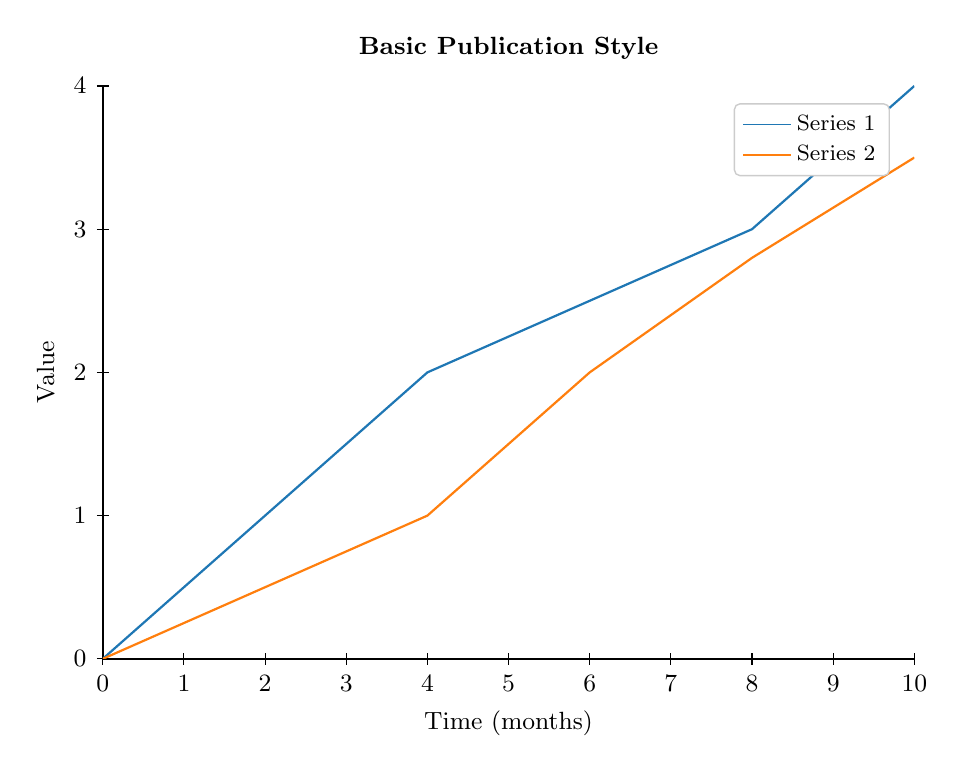
\begin{tikzpicture}
    \begin{axis}[
      publication,
      xlabel={Time (months)},
      ylabel={Value},
      title={Basic Publication Style}
    ]
      \addplot[primary] coordinates {(0,0) (2,1) (4,2) (6,2.5) (8,3) (10,4)};
      \addlegendentry{Series 1}
      \addplot[secondary] coordinates {(0,0) (2,0.5) (4,1) (6,2) (8,2.8) (10,3.5)};
      \addlegendentry{Series 2}
    \end{axis}
  \end{tikzpicture}
  \caption{Example of the basic publication style.}
\end{figure}

\subsection{Grid Variants}

\begin{figure}[ht]
  \centering
  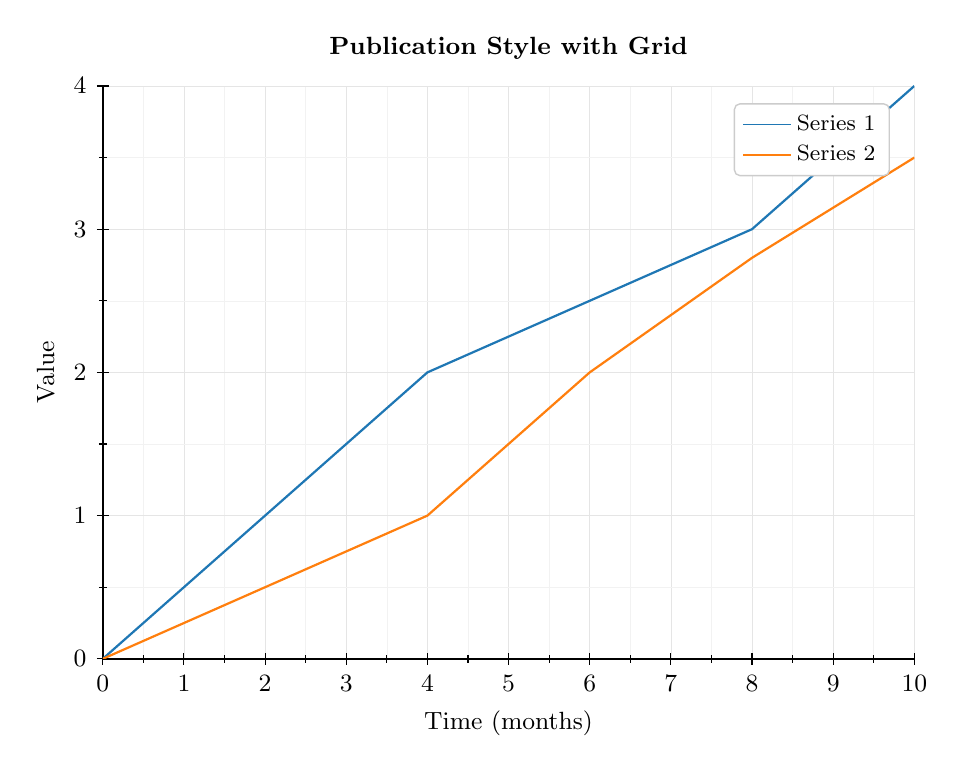
\begin{tikzpicture}
    \begin{axis}[
      publication grid,
      xlabel={Time (months)},
      ylabel={Value},
      title={Publication Style with Grid}
    ]
      \addplot[primary] coordinates {(0,0) (2,1) (4,2) (6,2.5) (8,3) (10,4)};
      \addlegendentry{Series 1}
      \addplot[secondary] coordinates {(0,0) (2,0.5) (4,1) (6,2) (8,2.8) (10,3.5)};
      \addlegendentry{Series 2}
    \end{axis}
  \end{tikzpicture}
  \caption{Example with grid lines for better readability.}
\end{figure}

\begin{multicols}{2}
\begin{figure}[H]
  \centering
  \begin{tikzpicture}
    \begin{axis}[
      publication grid x,
      xlabel={Time (months)},
      ylabel={Value},
      title={With X Grid}
    ]
      \addplot[primary] coordinates {(0,0) (2,1) (4,2) (6,2.5) (8,3) (10,4)};
    \end{axis}
  \end{tikzpicture}
  \caption{Grid on x-axis only.}
\end{figure}

\begin{figure}[H]
  \centering
  \begin{tikzpicture}
    \begin{axis}[
      publication grid y,
      xlabel={Time (months)},
      ylabel={Value},
      title={With Y Grid}
    ]
      \addplot[secondary] coordinates {(0,0) (2,0.5) (4,1) (6,2) (8,2.8) (10,3.5)};
    \end{axis}
  \end{tikzpicture}
  \caption{Grid on y-axis only.}
\end{figure}
\end{multicols}

\section{Survival Analysis Plots}

\subsection{Survival Curves}

\begin{figure}[ht]
  \centering
  \begin{tikzpicture}
    \begin{axis}[
      survival plot,
      title={Kaplan-Meier Survival Estimates},
      cycle list name=publishcolors
    ]
      \addplot+[solid] coordinates {
        (0, 1) (5, 0.95) (10, 0.85) (15, 0.70) (20, 0.60) (25, 0.55) (30, 0.50)
      };
      \addlegendentry{Treatment Group}
      
      \addplot+[solid] coordinates {
        (0, 1) (5, 0.90) (10, 0.75) (15, 0.60) (20, 0.45) (25, 0.35) (30, 0.30)
      };
      \addlegendentry{Control Group}
      
      % Add censoring marks
      \addplot+[only marks, mark=x, mark size=3pt, censoringColor] coordinates {
        (8, 0.87) (19, 0.63) (22, 0.58) (27, 0.52)
      };
      \addlegendentry{Censored}
      
      \addplot+[only marks, mark=x, mark size=3pt, censoringColor] coordinates {
        (6, 0.83) (17, 0.53) (21, 0.43) (28, 0.32)
      };
      \addlegendentry{}
    \end{axis}
  \end{tikzpicture}
  \caption{Example of survival curves showing treatment vs control group with censoring marks.}
\end{figure}

\subsection{Confidence Intervals}

\begin{figure}[ht]
  \centering
  \begin{tikzpicture}
    \begin{axis}[
      confidence interval plot,
      title={Survival with 95\% Confidence Interval}
    ]
      \addplot[primary, thick, name path=main] coordinates {
        (0, 1) (5, 0.95) (10, 0.85) (15, 0.70) (20, 0.60) (25, 0.55) (30, 0.50)
      };
      \addlegendentry{Survival}
      
      \addplot[primary!40, custom dashed, name path=upper] coordinates {
        (0, 1) (5, 0.98) (10, 0.92) (15, 0.80) (20, 0.72) (25, 0.68) (30, 0.63)
      };
      \addlegendentry{95\% CI Upper}
      
      \addplot[primary!40, custom dashed, name path=lower] coordinates {
        (0, 1) (5, 0.91) (10, 0.78) (15, 0.60) (20, 0.48) (25, 0.42) (30, 0.37)
      };
      \addlegendentry{95\% CI Lower}
      
      \addplot[confidence band] fill between[of=upper and lower];
    \end{axis}
  \end{tikzpicture}
  \caption{Survival curve with confidence intervals shown as a shaded band.}
\end{figure}

\subsection{Competing Risks (MENSA)}

\begin{figure}[ht]
  \centering
  \begin{tikzpicture}
    \begin{axis}[
      mensa plot,
      title={Cumulative Incidence Functions - Competing Risks}
    ]
      % Event 1
      \addplot[event1Color, thick] coordinates {
        (0, 0) (5, 0.05) (10, 0.15) (15, 0.30) (20, 0.40) (25, 0.45) (30, 0.50)
      };
      \addlegendentry{Event 1}
      
      % Event 2
      \addplot[event2Color, thick] coordinates {
        (0, 0) (5, 0.03) (10, 0.07) (15, 0.12) (20, 0.18) (25, 0.22) (30, 0.25)
      };
      \addlegendentry{Event 2}
      
      % Event 3
      \addplot[event3Color, thick] coordinates {
        (0, 0) (5, 0.02) (10, 0.05) (15, 0.08) (20, 0.10) (25, 0.12) (30, 0.15)
      };
      \addlegendentry{Event 3}
      
      % Overall cumulative incidence
      \addplot[octonaryDark, thick, custom dashed] coordinates {
        (0, 0) (5, 0.10) (10, 0.27) (15, 0.50) (20, 0.68) (25, 0.79) (30, 0.90)
      };
      \addlegendentry{Overall}
    \end{axis}
  \end{tikzpicture}
  \caption{Competing risks model showing cumulative incidence for different event types.}
\end{figure}

\subsection{Risk Stratification}

\begin{figure}[ht]
  \centering
  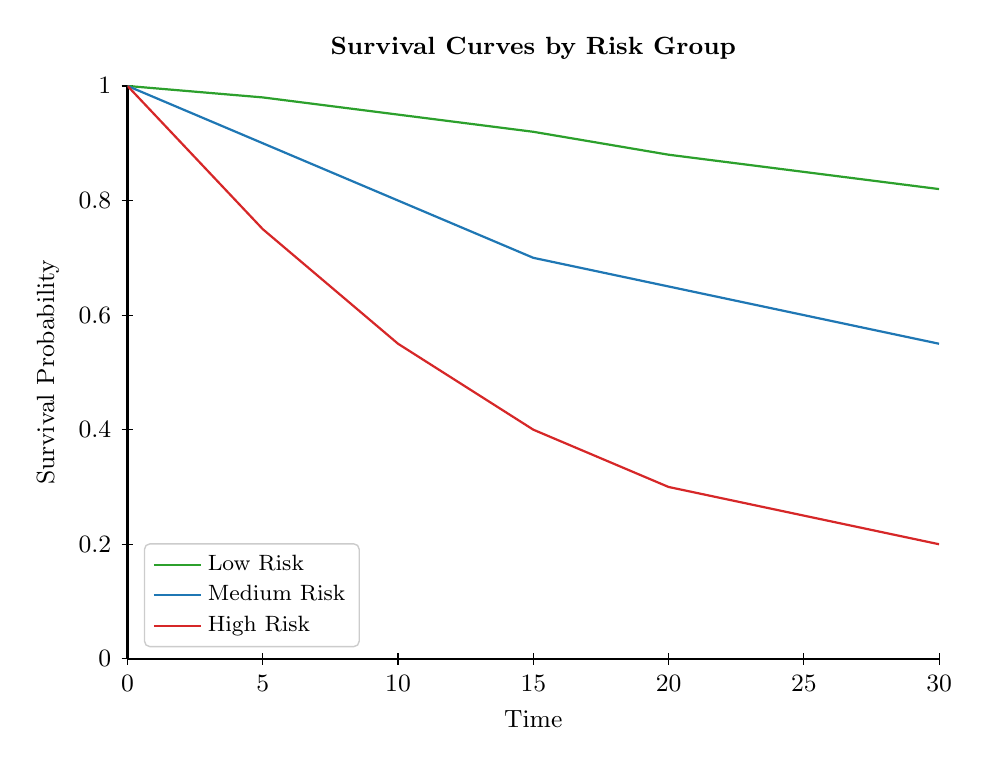
\begin{tikzpicture}
    \begin{axis}[
      risk stratification,
      title={Survival Curves by Risk Group}
    ]
      % Low risk
      \addplot[lowRiskColor, thick] coordinates {
        (0, 1) (5, 0.98) (10, 0.95) (15, 0.92) (20, 0.88) (25, 0.85) (30, 0.82)
      };
      \addlegendentry{Low Risk}
      
      % Medium risk
      \addplot[mediumRiskColor, thick] coordinates {
        (0, 1) (5, 0.90) (10, 0.80) (15, 0.70) (20, 0.65) (25, 0.60) (30, 0.55)
      };
      \addlegendentry{Medium Risk}
      
      % High risk
      \addplot[highRiskColor, thick] coordinates {
        (0, 1) (5, 0.75) (10, 0.55) (15, 0.40) (20, 0.30) (25, 0.25) (30, 0.20)
      };
      \addlegendentry{High Risk}
    \end{axis}
  \end{tikzpicture}
  \caption{Risk stratification showing survival curves for different risk groups.}
\end{figure}

\section{Deep Survival Machine Plots}

\begin{figure}[ht]
  \centering
  \begin{tikzpicture}
    \begin{axis}[
      dsm plot,
      title={Density Mixture Components in DSM},
      domain=0:15
    ]
      % Individual mixture components
      \addplot[name path=c1, likelihoodLossColor, thick, domain=0:15, samples=100] {0.5*exp(-(x-3)^2/4)};
      \addlegendentry{Component 1}
      
      \addplot[name path=c2, rankingLossColor, thick, domain=0:15, samples=100] {0.3*exp(-(x-7)^2/3)};
      \addlegendentry{Component 2}
      
      \addplot[name path=c3, regressionLossColor, thick, domain=0:15, samples=100] {0.2*exp(-(x-11)^2/5)};
      \addlegendentry{Component 3}
      
      % Overall mixture density
      \addplot[black, custom ultra thick, domain=0:15, samples=100] {0.5*exp(-(x-3)^2/4) + 0.3*exp(-(x-7)^2/3) + 0.2*exp(-(x-11)^2/5)};
      \addlegendentry{Mixture}
    \end{axis}
  \end{tikzpicture}
  \caption{Deep Survival Machine (DSM) mixture density components.}
\end{figure}

\section{Training and Evaluation Plots}

\subsection{Loss Function Comparison}

\begin{figure}[ht]
  \centering
  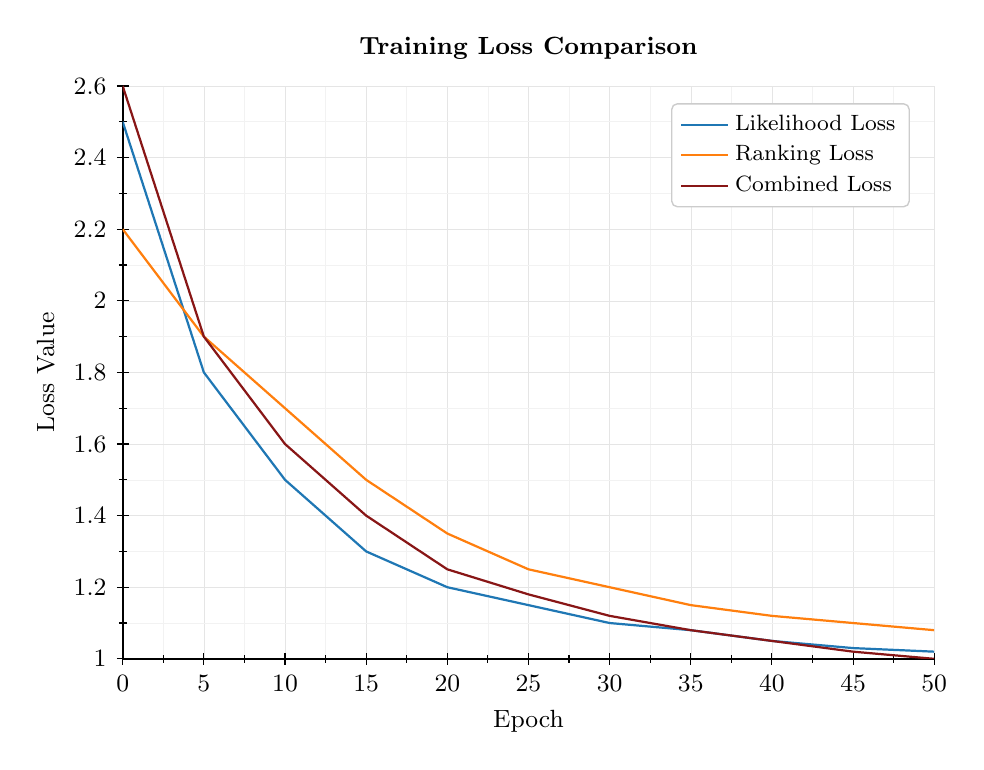
\begin{tikzpicture}
    \begin{axis}[
      loss comparison,
      title={Training Loss Comparison}
    ]
      % NLL Loss
      \addplot[likelihoodLossColor, thick] coordinates {
        (0, 2.5) (5, 1.8) (10, 1.5) (15, 1.3) (20, 1.2) 
        (25, 1.15) (30, 1.1) (35, 1.08) (40, 1.05) (45, 1.03) (50, 1.02)
      };
      \addlegendentry{Likelihood Loss}
      
      % Ranking Loss
      \addplot[rankingLossColor, thick] coordinates {
        (0, 2.2) (5, 1.9) (10, 1.7) (15, 1.5) (20, 1.35) 
        (25, 1.25) (30, 1.2) (35, 1.15) (40, 1.12) (45, 1.1) (50, 1.08)
      };
      \addlegendentry{Ranking Loss}
      
      % Combined Loss
      \addplot[quaternaryDark, thick] coordinates {
        (0, 2.6) (5, 1.9) (10, 1.6) (15, 1.4) (20, 1.25) 
        (25, 1.18) (30, 1.12) (35, 1.08) (40, 1.05) (45, 1.02) (50, 1.0)
      };
      \addlegendentry{Combined Loss}
    \end{axis}
  \end{tikzpicture}
  \caption{Comparison of training loss curves for different loss functions.}
\end{figure}

\subsection{Calibration Plot}

\begin{figure}[ht]
  \centering
  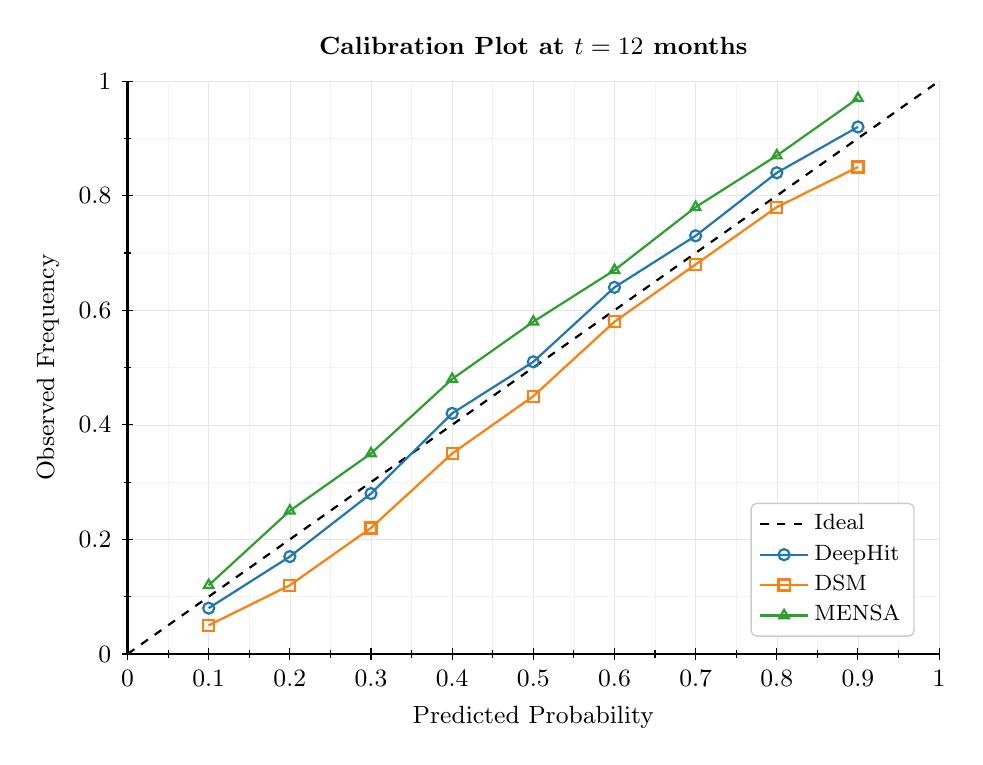
\begin{tikzpicture}
    \begin{axis}[
      calibration plot,
      title={Calibration Plot at $t=12$ months}
    ]
      % Reference line
      \addplot[black, custom dashed] coordinates {(0,0) (1,1)};
      \addlegendentry{Ideal}
      
      % Model 1 calibration 
      \addplot[primary, thick, mark=o] coordinates {
        (0.1, 0.08) (0.2, 0.17) (0.3, 0.28) (0.4, 0.42) 
        (0.5, 0.51) (0.6, 0.64) (0.7, 0.73) (0.8, 0.84) (0.9, 0.92)
      };
      \addlegendentry{DeepHit}
      
      % Model 2 calibration
      \addplot[secondary, thick, mark=square] coordinates {
        (0.1, 0.05) (0.2, 0.12) (0.3, 0.22) (0.4, 0.35) 
        (0.5, 0.45) (0.6, 0.58) (0.7, 0.68) (0.8, 0.78) (0.9, 0.85)
      };
      \addlegendentry{DSM}
      
      % Model 3 calibration
      \addplot[tertiary, thick, mark=triangle] coordinates {
        (0.1, 0.12) (0.2, 0.25) (0.3, 0.35) (0.4, 0.48) 
        (0.5, 0.58) (0.6, 0.67) (0.7, 0.78) (0.8, 0.87) (0.9, 0.97)
      };
      \addlegendentry{MENSA}
    \end{axis}
  \end{tikzpicture}
  \caption{Calibration plot comparing predicted vs. observed probabilities.}
\end{figure}

\section{Hazard Functions}

\begin{figure}[ht]
  \centering
  \begin{tikzpicture}
    \begin{axis}[
      hazard plot,
      title={Estimated Hazard Functions},
      ymax=0.15
    ]
      % Weibull hazard
      \addplot[primary, thick, domain=0:20, samples=100] {0.05*1.2*(0.05*x)^(1.2-1)};
      \addlegendentry{Weibull ($\lambda=0.05,k=1.2$)}
      
      % Gompertz hazard
      \addplot[secondary, thick, domain=0:20, samples=100] {0.01*exp(0.1*x)};
      \addlegendentry{Gompertz ($\alpha=0.01,\beta=0.1$)}
      
      % Log-normal hazard approximation
      \addplot[tertiary, thick, domain=0.1:20, samples=100] 
        {exp(-0.5*((ln(x)-1.5)/0.8)^2)/(x*0.8*sqrt(2*pi))/
         (1-0.5*(1+erf((ln(x)-1.5)/(0.8*sqrt(2)))))};
      \addlegendentry{Log-normal ($\mu=1.5,\sigma=0.8$)}
      
      % Bathtub hazard (composite)
      \addplot[quaternary, thick, domain=0:20, samples=100] 
        {0.1*exp(-0.5*x) + 0.01 + 0.002*x^1.5};
      \addlegendentry{Bathtub}
    \end{axis}
  \end{tikzpicture}
  \caption{Different hazard functions used in survival analysis.}
\end{figure}

\section{Performance Comparison}

\begin{figure}[ht]
  \centering
  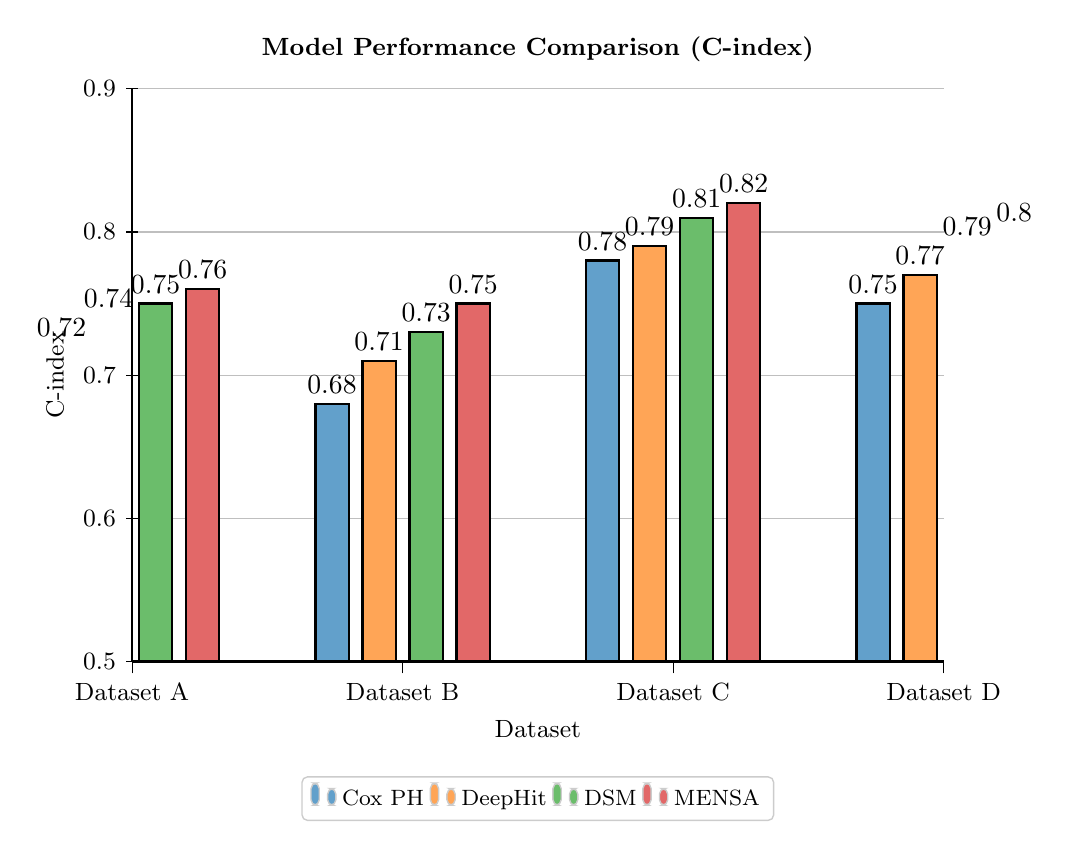
\begin{tikzpicture}
    \begin{axis}[
      publication,
      title={Model Performance Comparison (C-index)},
      xlabel={Dataset},
      ylabel={C-index},
      ybar=5pt,
      ymajorgrids=true,
      bar width=12pt,
      ymin=0.5, ymax=0.9,
      symbolic x coords={Dataset A, Dataset B, Dataset C, Dataset D},
      xtick=data,
      nodes near coords,
      nodes near coords align={vertical},
      legend style={at={(0.5,-0.2)}, anchor=north, legend columns=-1}
    ]
      \addplot[fill=primary!70] coordinates {
        (Dataset A, 0.72) (Dataset B, 0.68) (Dataset C, 0.78) (Dataset D, 0.75)
      };
      \addlegendentry{Cox PH}
      
      \addplot[fill=secondary!70] coordinates {
        (Dataset A, 0.74) (Dataset B, 0.71) (Dataset C, 0.79) (Dataset D, 0.77)
      };
      \addlegendentry{DeepHit}
      
      \addplot[fill=tertiary!70] coordinates {
        (Dataset A, 0.75) (Dataset B, 0.73) (Dataset C, 0.81) (Dataset D, 0.79)
      };
      \addlegendentry{DSM}
      
      \addplot[fill=quaternary!70] coordinates {
        (Dataset A, 0.76) (Dataset B, 0.75) (Dataset C, 0.82) (Dataset D, 0.80)
      };
      \addlegendentry{MENSA}
    \end{axis}
  \end{tikzpicture}
  \caption{Comparison of models across different datasets using C-index.}
\end{figure}

\section{Combined Plot Examples}

\begin{figure}[ht]
  \centering
  \begin{tikzpicture}
    \begin{axis}[
      publication,
      width=0.85\textwidth,
      height=8cm,
      title={Multiple Performance Metrics},
      xlabel={$\lambda$ (Regularization)},
      ylabel={Performance},
      xmode=log,
      log basis x=10,
      xmin=0.0001, xmax=10,
      legend pos=north east,
      grid=both,
      grid style={octonary!20, very thin},
      cycle list name=publishcolors
    ]
      % C-index
      \addplot+[thick] coordinates {
        (0.0001, 0.82) (0.001, 0.83) (0.01, 0.84) (0.1, 0.85) 
        (0.5, 0.83) (1, 0.81) (5, 0.75) (10, 0.70)
      };
      \addlegendentry{C-index}
      
      % Integrated Brier Score
      \addplot+[thick] coordinates {
        (0.0001, 0.25) (0.001, 0.23) (0.01, 0.20) (0.1, 0.18) 
        (0.5, 0.19) (1, 0.22) (5, 0.28) (10, 0.33)
      };
      \addlegendentry{IBS (scaled)}
      
      % Log-likelihood
      \addplot+[thick] coordinates {
        (0.0001, 0.60) (0.001, 0.65) (0.01, 0.70) (0.1, 0.78) 
        (0.5, 0.75) (1, 0.70) (5, 0.60) (10, 0.55)
      };
      \addlegendentry{NLL (scaled)}
      
      % Optimal point annotation
      \draw[red, custom dashed] (axis cs:0.1,0) -- (axis cs:0.1,1);
      \node[align=center, font=\small, text=quaternaryDark, rotate=90] at (axis cs:0.1,0.5) 
        {Optimal $\lambda$};
    \end{axis}
  \end{tikzpicture}
  \caption{Comprehensive view of multiple performance metrics across different regularization values.}
\end{figure}

\end{document}